\documentclass[11pt]{article}
\usepackage[textwidth=18.0cm, textheight=23.0cm, top=2.0cm]{geometry}
\usepackage{pst-all}
\usepackage{amssymb}
\usepackage{tikz}
\usepackage{underscore}\begin{document}
\pagestyle{empty}


ClassName: \underline{\textbf{Class_10.2bp-2}}
\par
BinSize: \underline{\textbf{100 × 100}}
\par
ReduceSize: \underline{\textbf{100 × 100}}
\par
TypeNum: \underline{\textbf{20}}
\par
Num: \underline{\textbf{20}}
\par
OutS: \underline{\textbf{40000}}
\par
InS: \underline{\textbf{35461}}
\par
Rate: \underline{\textbf{0.887}}
\par
UB: \underline{\textbf{4}}
\par
LB0: \underline{\textbf{4}}
\par
LB: \underline{\textbf{4}}
\par
LBWithCut: \underline{\textbf{4}}
\par
NodeCut: \underline{\textbf{0}}
\par
ExtendedNodeCnt: \underline{\textbf{1}}
\par
GenNodeCnt: \underline{\textbf{1}}
\par
PrimalNode: \underline{\textbf{0}}
\par
ColumnCount: \underline{\textbf{4}}
\par
TotalCutCount: \underline{\textbf{0}}
\par
RootCutCount: \underline{\textbf{0}}
\par
LPSolverCnt: \underline{\textbf{1}}
\par
PricingSolverCnt: \underline{\textbf{0}}
\par
BranchAndBoundNum: \underline{\textbf{1}}
\par
isOpt: \underline{\textbf{true}}
\par
TimeOnPrimal: \underline{\textbf{0.000 s}}
\par
TimeOnPricing: \underline{\textbf{0.000 s}}
\par
TimeOnRmp: \underline{\textbf{0.078 s}}
\par
TotalTime: \underline{\textbf{0.125 s}}
\par
\newpage


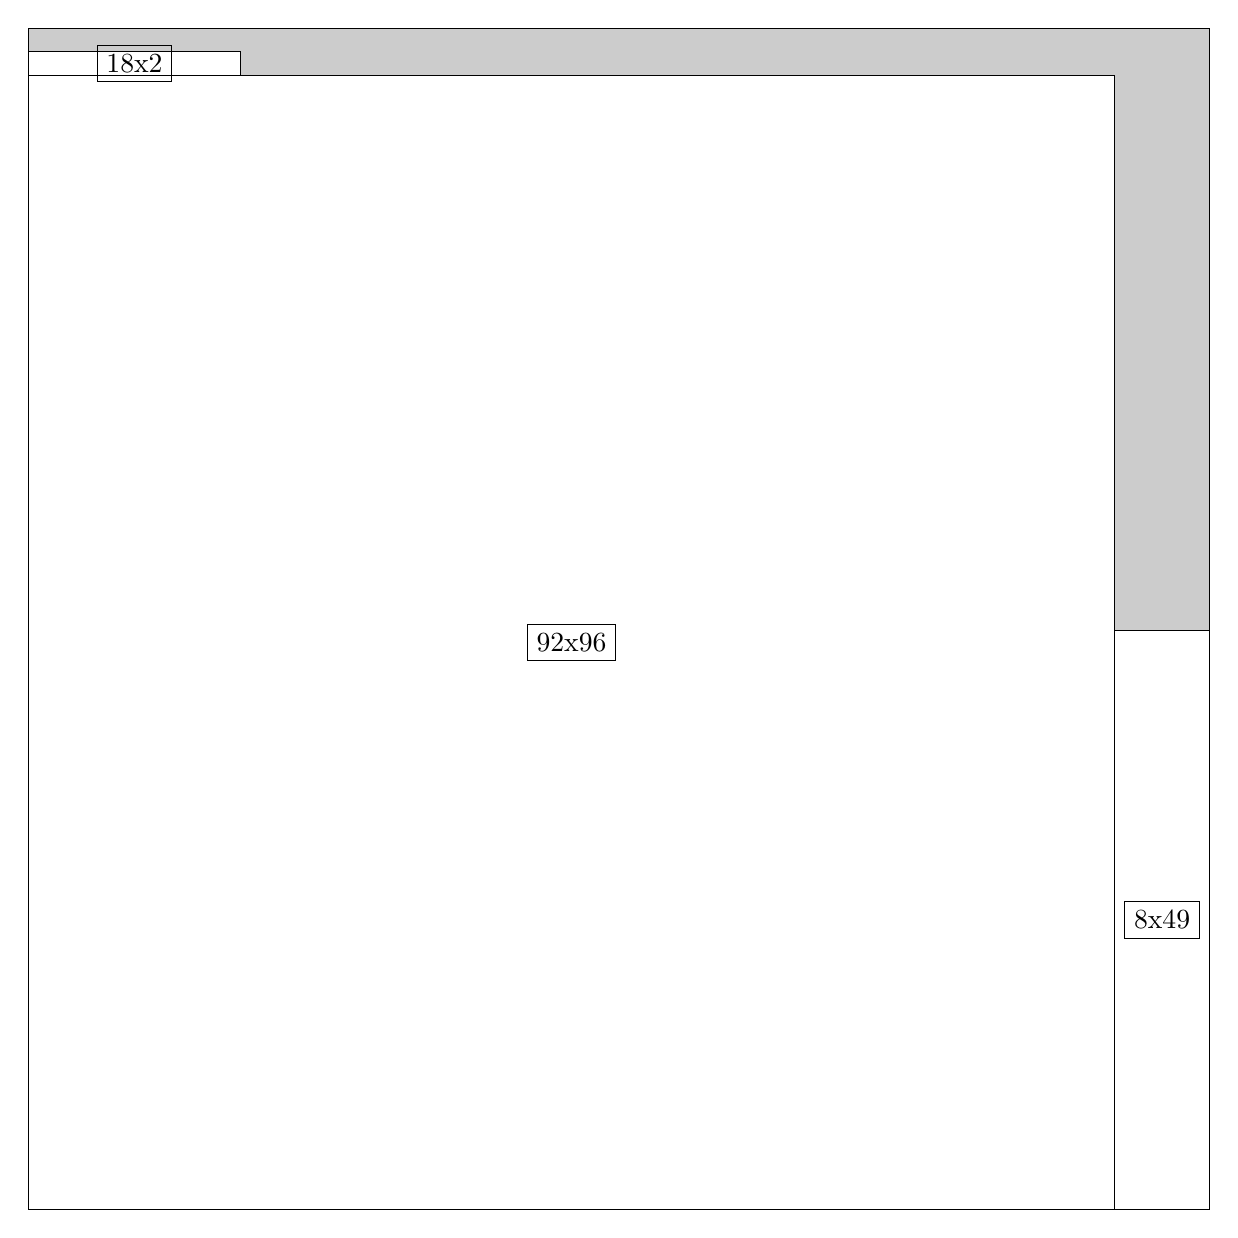
\begin{tikzpicture}[shorten >=1pt,scale=1.0,every node/.style={scale=1.0},->]
\tikzstyle{vertex}=[circle,fill=black!25,minimum size=14pt,inner sep=0pt]
\filldraw[fill=gray!40!white, draw=black] (0,0) rectangle (15.0,15.0);
\foreach \name/\x/\y/\w/\h in {92x96/0.0/0.0/13.799999999999999/14.399999999999999,18x2/0.0/14.399999999999999/2.6999999999999997/0.3,8x49/13.799999999999999/0.0/1.2/7.35}
\filldraw[fill=white!40!white, draw=black] (\x,\y) rectangle node[draw] (\name) {\name} ++(\w,\h);
\end{tikzpicture}


w =92 , h =96 , x =0 , y =0 , v =8832
\par
w =18 , h =2 , x =0 , y =96 , v =36
\par
w =8 , h =49 , x =92 , y =0 , v =392
\par
\newpage


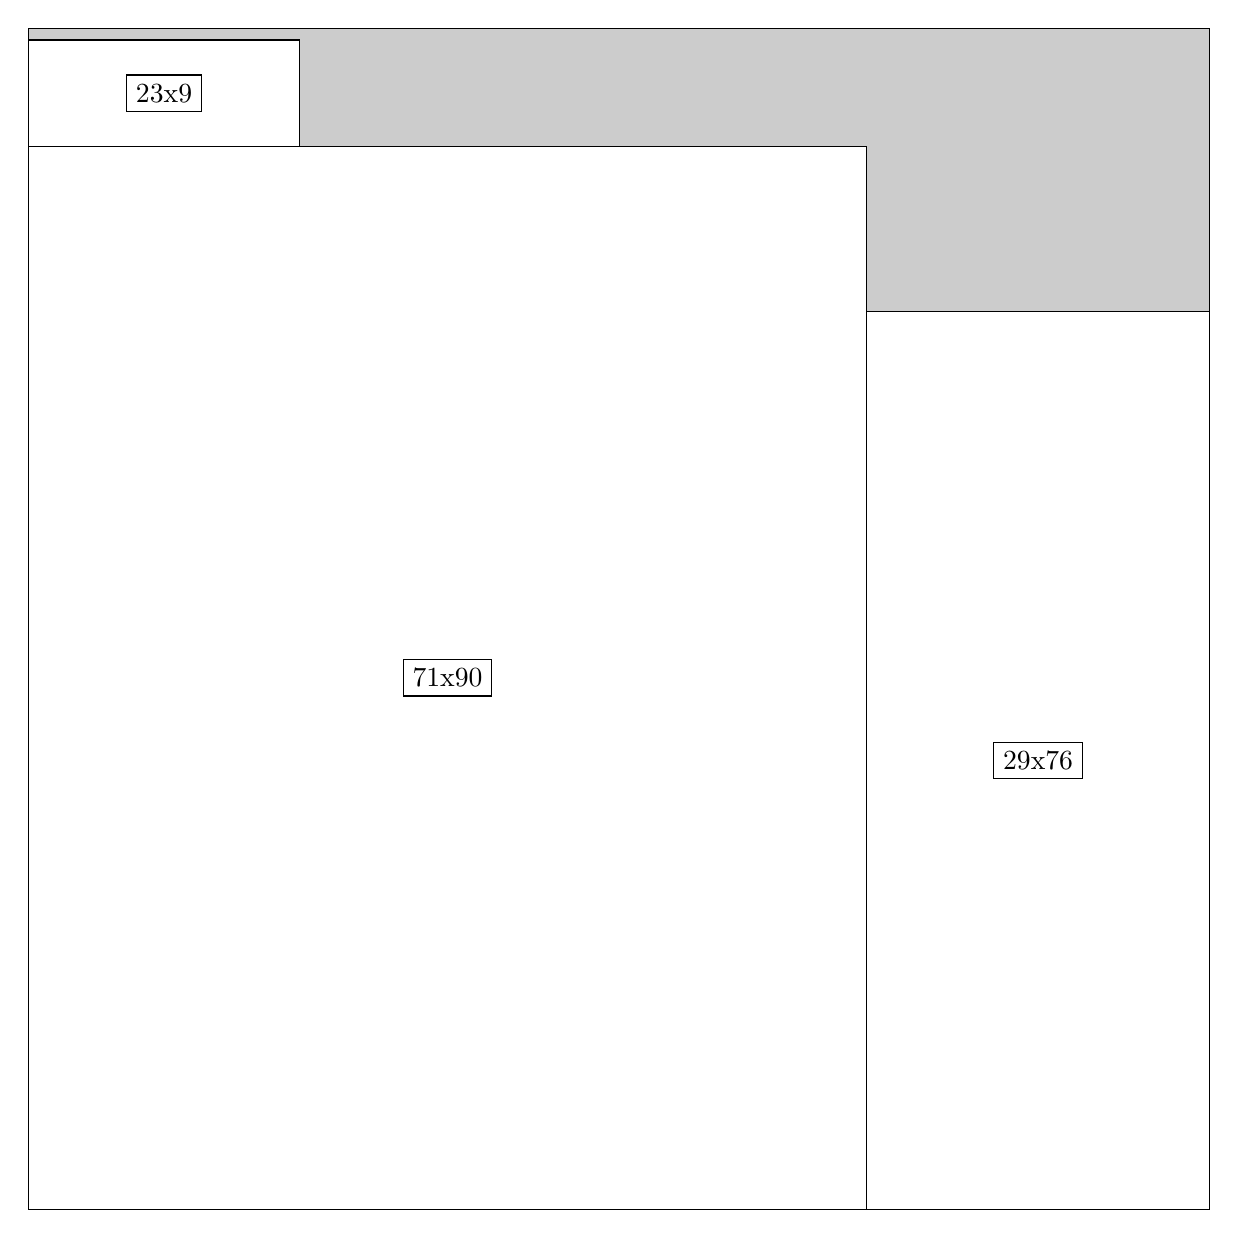
\begin{tikzpicture}[shorten >=1pt,scale=1.0,every node/.style={scale=1.0},->]
\tikzstyle{vertex}=[circle,fill=black!25,minimum size=14pt,inner sep=0pt]
\filldraw[fill=gray!40!white, draw=black] (0,0) rectangle (15.0,15.0);
\foreach \name/\x/\y/\w/\h in {71x90/0.0/0.0/10.65/13.5,29x76/10.65/0.0/4.35/11.4,23x9/0.0/13.5/3.4499999999999997/1.3499999999999999}
\filldraw[fill=white!40!white, draw=black] (\x,\y) rectangle node[draw] (\name) {\name} ++(\w,\h);
\end{tikzpicture}


w =71 , h =90 , x =0 , y =0 , v =6390
\par
w =29 , h =76 , x =71 , y =0 , v =2204
\par
w =23 , h =9 , x =0 , y =90 , v =207
\par
\newpage


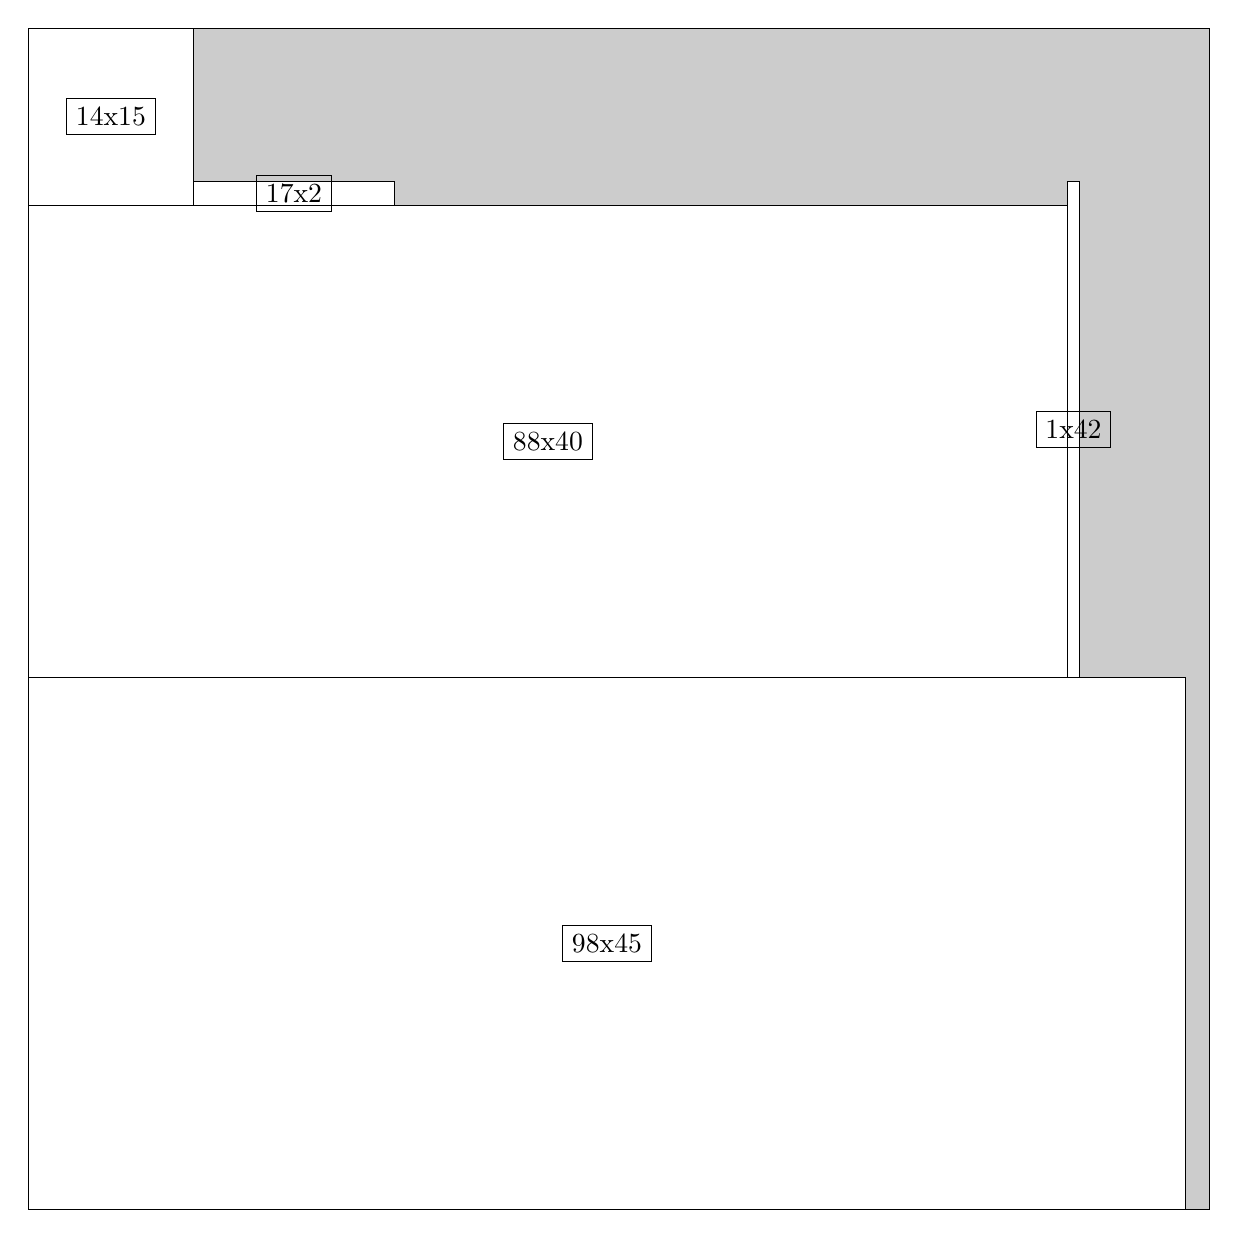
\begin{tikzpicture}[shorten >=1pt,scale=1.0,every node/.style={scale=1.0},->]
\tikzstyle{vertex}=[circle,fill=black!25,minimum size=14pt,inner sep=0pt]
\filldraw[fill=gray!40!white, draw=black] (0,0) rectangle (15.0,15.0);
\foreach \name/\x/\y/\w/\h in {98x45/0.0/0.0/14.7/6.75,88x40/0.0/6.75/13.2/6.0,14x15/0.0/12.75/2.1/2.25,1x42/13.2/6.75/0.15/6.3,17x2/2.1/12.75/2.55/0.3}
\filldraw[fill=white!40!white, draw=black] (\x,\y) rectangle node[draw] (\name) {\name} ++(\w,\h);
\end{tikzpicture}


w =98 , h =45 , x =0 , y =0 , v =4410
\par
w =88 , h =40 , x =0 , y =45 , v =3520
\par
w =14 , h =15 , x =0 , y =85 , v =210
\par
w =1 , h =42 , x =88 , y =45 , v =42
\par
w =17 , h =2 , x =14 , y =85 , v =34
\par
\newpage


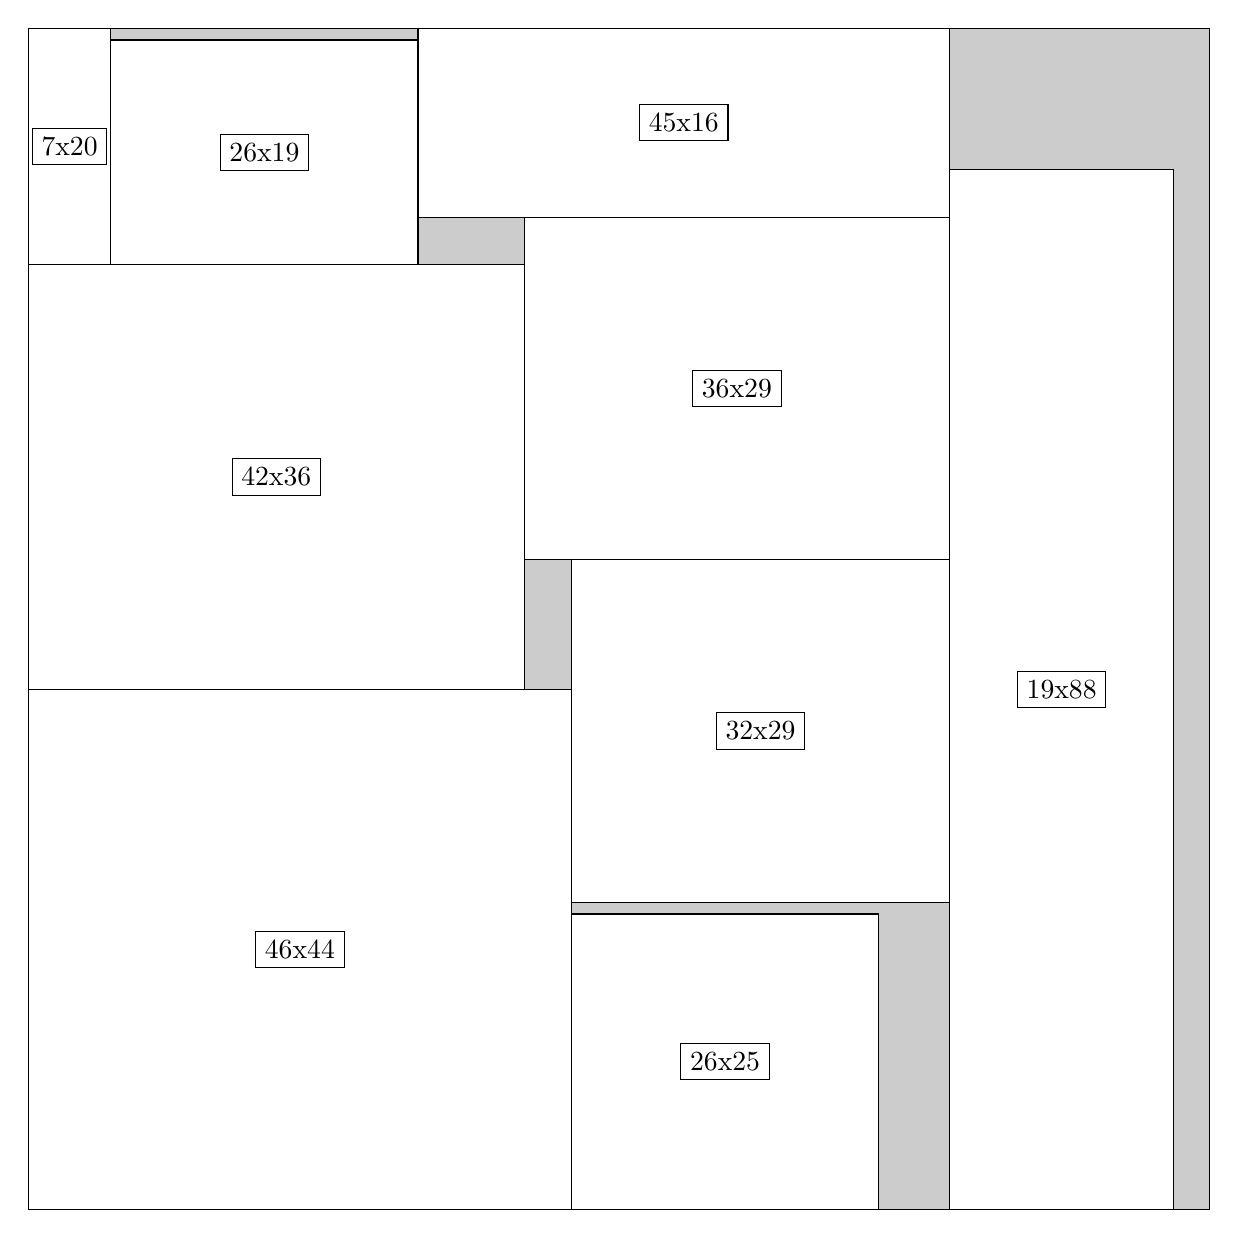
\begin{tikzpicture}[shorten >=1pt,scale=1.0,every node/.style={scale=1.0},->]
\tikzstyle{vertex}=[circle,fill=black!25,minimum size=14pt,inner sep=0pt]
\filldraw[fill=gray!40!white, draw=black] (0,0) rectangle (15.0,15.0);
\foreach \name/\x/\y/\w/\h in {46x44/0.0/0.0/6.8999999999999995/6.6,19x88/11.7/0.0/2.85/13.2,42x36/0.0/6.6/6.3/5.3999999999999995,32x29/6.8999999999999995/3.9/4.8/4.35,45x16/4.95/12.6/6.75/2.4,26x25/6.8999999999999995/0.0/3.9/3.75,26x19/1.05/12.0/3.9/2.85,7x20/0.0/12.0/1.05/3.0,36x29/6.3/8.25/5.3999999999999995/4.35}
\filldraw[fill=white!40!white, draw=black] (\x,\y) rectangle node[draw] (\name) {\name} ++(\w,\h);
\end{tikzpicture}


w =46 , h =44 , x =0 , y =0 , v =2024
\par
w =19 , h =88 , x =78 , y =0 , v =1672
\par
w =42 , h =36 , x =0 , y =44 , v =1512
\par
w =32 , h =29 , x =46 , y =26 , v =928
\par
w =45 , h =16 , x =33 , y =84 , v =720
\par
w =26 , h =25 , x =46 , y =0 , v =650
\par
w =26 , h =19 , x =7 , y =80 , v =494
\par
w =7 , h =20 , x =0 , y =80 , v =140
\par
w =36 , h =29 , x =42 , y =55 , v =1044
\par
\newpage


\end{document}